\documentclass[10pt,a4paper]{report}

\usepackage[utf8]{inputenc}
\usepackage{amsmath}
\usepackage{amsfonts}
\usepackage{amssymb}
\usepackage{graphicx}
\usepackage{hyperref}
\usepackage{lstlisting}
\usepackage[left=2cm,right=2cm,top=2cm,bottom=2cm]{geometry}

\title{Title}
\author{Programming Life group 2\\
	\begin{tabular}{c c c}
	\hline 
		Derk-Jan Karrenbeld & 4021967 & 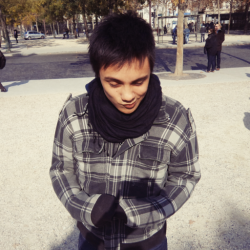
\includegraphics[scale=0.2]{../img/DJ.png}\\ 
		Joost Verdoorn & 1545396 & 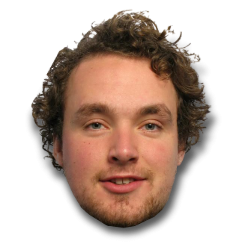
\includegraphics[scale=0.2]{../img/Yoloost.png}\\ 
		Steffan Sluis & 4088816 & 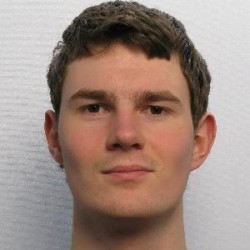
\includegraphics[scale=0.2]{../img/SS.jpeg}\\ 
		Tung Phan & 4004868 & 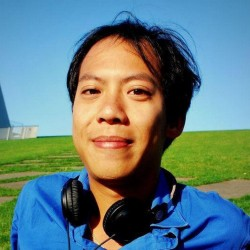
\includegraphics[scale=0.2]{../img/TP.jpeg}\\ 
		Vincent Robbemond & 4174097 & 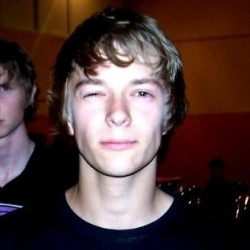
\includegraphics[scale=0.2]{../img/VR.jpeg}\\ 
		\hline 
	\end{tabular} 
}
\date{\today}

\begin{document}
	\maketitle

	\setcounter{section}{0}
	\setcounter{secnumdepth}{3}
	\setcounter{tocdepth}{5}
	\renewcommand*\thesection{\arabic{section}}
	
	\pdfbookmark{\contentsname}{toc}
	\tableofcontents

	\clearpage

	\section{Introduction}
		This is the Draft Final Report for the Context Project: Programming Life.\\
		During this project we have built Gigabase, an app to create the virtual cell. The creation of this application was not without its challenges, but as a team we managed to overcome these and together we didn't only work towards a great product, we also grew as individuals, refined our personalities when it comes to teamwork and had a lot of fun.\\
		This document reflects on these challenges, that teamwork and what the project itself means to us.
		
	\section{Key challenges and Solutions}
		The project itself had some challenges that were conceived as difficult. Apart from these challenges, the process itself had some as well, which are listed under 'Reflection on the teamwork'. 
		
		\subsection{ODE modularity}
			Let's first define component as any module or metabolite in the cell such as a transporter or substrate. The biological-cell model consists of components that interact with eachother, but the differential equations are not defined by interaction, but component. Our task was to make these components modular, meaning you need to be able to change them, add more of them and so forth and so on. But since these differential equations were intertwined, a way needed to be devised to seperate them and make the arguments dynamic. For example '\frac{ds}{dt} = ks * s + kc * c' would need to assign s and c dynamically. kc belongs to c, so it's probably its own compound. If we have two, it would become '\frac{ds}{dt} = ks * s + kc1 * c1 + kc2 * c2'.\\
			We wrote a mapping code that collects produced compounds. So c would produce c and s and s would produce s. The equations were seperated by how operators depencies work. We gave each compound all the effects and affects as equations. s now has '\frac{ds}{dt} = ks * s' and c has '\frac{ds}{dt} = kc * c' and '\frac{dc}{dt} = magix' Now adding more c's will dynamically build the correct equation. But since we have a mapping, we can use indexes to get those compound values. '\frac{ds}{dt} = ks * compounds[s]'. And if we make the indexer a settable parameter, we are done! '\frac{ds}{dt} = @ks * compounds[@s]'. \\
			This way we could turn the equations from statically defined to dynamically settable.
			
		\subsection{ODE solver complexity}
			Our ordinary differential equations solver is the same used in MATLAB. It's very powerfull but this did yield some problems. The more components we added, the more noticeable the delay between pressing simulate and the actual output. To get accurate results we were doing the caluclations on a low tolerance and a high number of iterations. \\
			One could always tweak this tolerance and iteration number, but defining that dynamically is hard. Instead we took a different road. We re-implemented the ODE by implementing the algorithm and deferring each iteration. This made the overal solving time higher, but there was no UI freeze anymore whatsoever. We could now also display results on the fly and show progress.\\
			If the next function denotes the pseudocode:\\
			\begin{lstlisting}
ODE Solver( T, f, y, I )
	initialize t = 0, y = [ y ], i = 0
	WHILE t \lt T AND i \lt I
		WHILE error \gt tolerance
			6 times solve dopri f()
			determine error
			increment i
		y[ t ] = solved values
		increment t
			\end{lstlising}
			The outer while block was deferred. Deferring in JavaScript is achieved by pushing a function to the end of the callstack, using setTimeout.
		
		\subsection{Concurrency}
			The database operations themself are atomic: isolated, but since users can edit the same cell, or might have a copy on their local storage which isn't updated back into the database, consistency between data is a problem. We offer two solutions to the problem.\\ 
			
			Firstly there is a clone cell feature, where all the data is copied, rather than simply loaded. This means that you are safe editing that data. See it as forking a repository on GitHub.\\
			
			Secondly one can create access keys to his or her creation. This will make the cell readonly for everyone, unless they have the access key. This can also be used to create private cells, which have a limited amount of read-only access keys.
		
		\subsection{Offline availability}
			The application should be available offline. As this was one of our design goals, we chose to write the base functionality in a client side application. The next step was making this available to the offline user.\\
			HTML5 has new functionality with application manifests. We implemented these to make sure the application is available offline. The HTML5 Local Storage feature was used for a key-value database storage client side. The HTML5 online-offline events perfectly provided the link to transparently update both the database, as well as the application when a user came online.\\
			The beauty of this solution is that you don't need to install anything and the application simply degrades to online-only if these features are not available.
		
		\subsection{Undo}
			The ability to undo and redo your actions makes an interface more user friendly and easy to use, and so the decision to add this functionality to our application was made early on. This resulted in a functionality that could be added to as the application grew in complexity. The challenge in accomplishing this, is to store and update the relevant data in such a way in becomes a self containing entity. To do this, the functionality needs to have an easy to use interface, while all the complex logic is contained within the entity itself.
			
			In implementing this, it becomes evident that the interface to the entity consists of it's basic functions; namely \emph{undo], \emph{redo}, and \emph{addAction}. Any action that can be undone and redone is stored a tree structure, each point in time containing a reference to the previous point and all the future point that emerged from that specific snapshot in time. This allows for multiple possible timelines, and makes this functionality more powerfull without adding much complexity to the use of it, because everything complicated is contained within the entity.

			In addition to creating an easy to use implementation, it is also required that the functionality remains simple even when the cell model is very complex. To easily maintain the timeline of the entire application, each module keeps track of it's own history and future and makes this data avaiable. The cell also track changes made to it and makes its timeline avaiable. Because of this separation, any part of the cell model can be adapted without having to think about the consequences of the changes to other parts of the model, allowing for easier development and generally higher quality software.
	
	\section{Reflection on the teamwork}
		
		\subsection{Preparation}
Toolchain, autodidact rails, coffeescript en ruby te leren. Coding guidelines en styles hebben opgezet. 
Contactmomenten
		
		\subsection{Meetings and contact}
Wekelijks sprint planning op de eerste dag van de workweek, dag van meeting met de ta, aan het einde van de werkweek, skype, weekend, avond, nacht, drebbelweg, pair programming. Facebook groep

		\subsection{Task delegation}
Taken self assignen, scrum master wisselde door, regelde de vergadering. Openstaand taken werken opgenomen door mensen met minder uur. Nooit een probleem met taken die ongewild waren en niemand was a-relaxt. 

		\subsection{Interpersonal communication}
Respect, geen negativiteit. Gebrek aan afleveren gaf verantwoordelijk. Voor vroege ontmoetingen was ere en problem, in het team opgelost door compensatiegedrag. Gezellig. Koffiepas! 

		\subsection{Problems and challenges}
Er wordt om hulp gevraagd. Naar elkaar toe komen om vragen te stellen over geproduceerde code. We zagen elkaar veel dus dat kon ook.
	Niveau verschil -> besproken, project taal was voor iedereen onbekend, geïsoleerde projecten, motavatiepraatjes.
Elkaars code niet kennen -> test code zelf en voor ander mans code schrijven, zodat je alles uiteindelijk kent. Door te pair programmen en vraag- en antwoord momentjes tijdens contactmomenten. Strict documenteren van functies/commentaar
			\subsubsection*{Downtime during exams}
				During our planning, the fact that no real work can be done during the exams was not taken into account. This lead to a two to three weeks of considerable slowdown of the project progress.\\
				Nonetheless, there were still short, weekly meetings with the teaching assistents. Immediately after the exams, a revised planning has been made and the lost time during those exams has been made up for.
			\subsubsection*{Differences in level of expertise}
				The group is comprised of members of different levels of expertise, so the decision was made to use a whole new programming language.\\ 
				By doing this, the people with less aptitude in programming can still keep up with the rest, as everyone else is also learning the ropes of this new language.\\
				To further close the gap between the experienced and inexperienced members of the group, pair wise programming was introduced to the group, so the members can ask questions on the spot when something wasn't clear.\\
				Members also had their isolated projects where they can work at their own pace. This way, the more adept programmers can develop the more elaborate features and the rest can focus on their own tasks, so they don't slow each other down.\\ 
				Every week during the meetings, there was a mandatory moment where each member had to explain what they did, what went good/bad and what they were planning to do for that week.\\ 
				By doing this, it's possible to ask each other for advice when they were stuck at a problem and thus help each other.
			\subsubsection*{Punctuality}
				A recurring problem in the group was the occasional early meeting. Some members had the tendicy to be tardy and thus keeping the rest of the group waiting. \\
				This wasn't really a problem, because every member made up for the lost time by working in their own time, be it during the day or night. \\
				Most of the time, members were late at the meetings because they were sleep deprived by coding all night long. So the tardiness is compensated, be it by working in their own free time or by bringing cake.
			\subsubsection*{Understanding each other's work}
				Because of the scale of the project, a high volume of code can be written in a short amount of time by 	different members of the group. Because of this, it's easy to lose track of each other's work. \\
				This is solved by allowing other members of the group to write test classes for each other. This way, every member is aware of the work done by other members and helps understand the code.

	\section{Individual reflections on the project}
		This section of the report contains the personal reflections of each of the team members. It contains every members perspective on the project, rather than the global experience of the group.
		\subsection{Derk-Jan Karrenbeld}
			Biology always intrigued me, apart from the asexual reproduction among plants. My favourite subjects have always been protein synthesis and genetics. I don't know why, but the gist of DNA being a blueprint for a product, where a biological computer turns templates into actual instances fascinated me. How do these parts work together. Why do they react the way they do and why does such a complex system keep working. There is so much to explore when it comes to our physiology and even more when you dig into the inner workings. And asking questions I did.\\

With mitosis, the chromosomes are shorted by a tiny amount. This affect is reversed with reproduction where a enzyme ensures the chromosomes telomeres to be lengthy. Could we solve this problem by creating a 'safe virus' that injects telomerase, the enzyme, into living cells? How many would you need? How would the substances behave? Would it cure some diseases we get when we are of age, because of the broken DNA? Or would it incur more cancerous cells, because faulty ones would be more healthy? But if we can build a virus that does such an incredible thing, can we use biology to solve the other world problems of diminishing natural resources, food and clean drinking water? \\

This brings us to today. Before I dived into this project, I always thought the questions and challenges mentioned above were best answered by the field of biotechnology. However the principles I was thought in my - even - younger years, seemed so sloppy to me. Cutting DNA of other organisms into pieces, and sealing them into yet different ones, hoping that the result yields a living cell that doesn't affect it's environment in any other way than intended. But now I know that there is a whole lot more these days. The things we can do combining biology, chemistry and engineering are incredible. I was intrigued and now I am enlightened. \\

Living with a rare form of lymphoma means that every biological break-through is important. This project made me feel like I could be part of one of those breakthroughs. Yes, I am actively considering this as a future path. I always said Computational Biology is awesome, but Bioinformatics might just be my piece of cake. Not only have I learned that there is more than a mechanical machine, I also feel like this project thought me so much more. Thinking about UX on a whole new level. Understanding mathematics in chemistry and linking that to biology. It's like all my knowledge is coming together. It's an eye opener.\\

Building life from scratch kind of feels like playing for God and that got me thinking. What if one day the application we designed would be able to turn the virtual cells into real biological computers? Does that yield a new era of creationists of a new order? Do we, as humanity, reached a level of understanding that we are now capable of shaping the world as we want it, rather than dabbling around with nature's natural gems. Why aren't all scientists of all fields constantly motivated by the scientific world to work together? Look at what we can do! We can do incredible things. And I want to be part of it - it kind of feels like I already am. Surely my experience feels like level prokaryote, but that just means that there is so much more to explore. Surely questions were answered, but I'm now left with a whole lot more.

		\subsection{Joost Verdoorn}
			Let me start off by being honest admitting that my opinion of this particular context and the assignment was not especially high. I always like to build something that will or could actually be used. The game context would have provided me with a project to create something like that, and for that I listed it as my first choice. The Programming Life context didn’t seem to offer such a chance. However, I still had my reasons for listing this context as my second choice. I find the scientific field of microbiology a very interesting one, even though I never took biology in high school beyond the 3rd grade. \\

Also, before being enrolled into a particular context, I had the desire to step away from the web for a change. I have built websites for a living and I wanted a ‘change of scenery’, and I believe that was the case for more members of the team. Interestingly enough, in the first meetings the team held we decided that we were going to build a web app. To keep the assignment a challenge, we decided we decided we would get our kicks by using platforms, tools and languages we hadn’t used before. And that was a blessing. \\

The best discovery for me is the language CoffeeScript. It’s an object-oriented, Ruby inspired language that is converted - by the server - into JavaScript which can be run in a normal web browser. It was able to turn my dislike of developing for the web around and made me find again the fun that I have when I really enjoy what I’m doing. Throughout the project I found that the more I understood CoffeeScript, the more fun I had and the more time and effort I put into the project. \\

Besides the new tools, this was the first time I - and I believe any of our team - have actually employed the Scrum workflow. It’s a very nice way to do your project planning, although we didn’t put all the effort into it to follow the process it by the letter. We didn’t assign a designated Scrum master but instead rotated around the roles so any team member would gain some experience into this process. Also, we didn’t maintain the sprint log an backlog as well as we could have. Estimations for sprint log items also gained a lot of accuracy through the sprints. \\

I realize during the project I have grown as a software developer and as a team member. The team was awesome: we were all eager to learn new things, not afraid to asks questions and clever enough to develop out-of-the-box solutions. I’ve also learnt a lot about the context: the provided seminars provided me with a lot of food for thought and have inspired many hours of browsing and clicking through Wikipedia in the hunt for more knowledge. Nature works in incredible ways, and the basic knowledge provided in the seminars have enabled me to further grasp some of the intriguing details.

		\subsection{Steffan Sluis}
				This project was really a great part of my life during the past half year. Because I had already completed most lab assignments of the second year courses, I had a lot of time to spare to work on the application. This resulted in many longs nights of debugging, refactoring and more debugging, most of the times along with one or more of my fellow group members. For me, this was basically a fun way to spend my time, because the group is one of the greatest groups I have ever worked with, and their dedication and motivation motivated me to return that favor, creating an in my opinion allround positive experience.\\

	The context of the project didn't invoke much of a reaction in me at first, mostly because I've never worked much in any area to do with Biology, but the title of the project and the idea of `Programing Life', actually influencing life by programming, did and still does sound quite cool. It's made me wonder about the possibilities that exist with the technoligies we have used and contributed to, and I think I would enjoy a career in Bioinformatics, even though it would never have guessed it would be one of my choices to begin with.\\

	One peculiar side effect that working on the project seemed to cause, was that I would find myself going to sleep with my head full of ideas on how to create new functionalities for the application or just ideas about cool software in general. This of course threw me into an upwards spiral of spending time working on the project, becoming more excited and as such spending even more time on the project. Overall I think this was a first for me, because usually in projects I get excited about it, but not this much.\\

	Another effect of the project was that suddenly everything even remotely related to bacterias or cells or products reminded me of our application, resulting in me showing and explaining what we had been working on recently to anybody fortunate enough to share in the conversation. All that explaining made me understand the context of the project better, making my interests in Biology and especially Bioinformatics grow.\\

	All in all, I have had a great time the past weeks, and I attribute that mostly the project. I learned a lot of new things and I had a lot of fun doing it, not to mention that in my opinion the end result was worth every bit of time put into it. I think it ultimately made me a better programmer and someone who is a little more informed on the inner workings of cells than most people.

		\subsection{Tung Phan}
				Before the project began, I had no idea what would be in store for me. I didn't know what bioinformatics was and, to be fair, it wasn't my first choice either. But I have zero regrets, as I've rediscovered my love for informatics and learned to view it from a different perspective. Thanks to the project, bioinformatics is also something I'll take into account when I'm choosing a master.\\

	The project taught me my limitations of an undergraduate, as my skills were more on the lacking side that I hoped. And that's okay. I learned to take stuff at my own pace, instead of constantly comparing my capabilities to others. That also reassures me that computer science is still the future for me, as for the past year, I had serious doubts about my choice and skills. I considered it a race, and I was losing it. I was constantly being amazed by other programmers my age, how they were completely out of my league and doubted my future. Due to help from a few team members, I finally realised, even though it sounds obvious, that I'm going to college for my own good. Not for my family, friends or future boss, but for myself. They reached this level of skill by dedication and hard work and not by some funny whim of nature, it's just that some people are quicker on the uptake than others and I'm fine with it.\\

	After experiencing what bioinformatics can do, I've been curious about the application of informatics in the world, combining different fields and forming a whole new field.\\

	As we worked with a whole new language in this project, I've learned to work outside my comfort zone, getting used to the new tools and developing environment. It has also urged me to learn more about said language, Ruby (on Rails), and this project made me want to work on personal projects in this language too.\\

	Lastly, this project has been a confirmation for what I want to do later in life as a computer scientist. I definitely belong in the higher level group of computer scientists: focussing more on developing software than, for example, optimising the programming languages. One of the things I want do to is to be able to develop software to help other fields effectively accomplish their goals.

		\subsection{Vincent Robbemond}
			Despite the fact Biology has always been one of my fields of interest I didn't do a lot with it up until this project. The context seminars definitely spiked my interest, especially because it brought biology and informatics together in the form of Bioinformatics. I never thought much about the application of informatics in other fields of study, so this was almost entirely new to me. I really enjoyed the modelling of a cell by means of programming, this shows the opportunities and capabilities of Bioinformatics, definitely something to remember and take into account when choosing a master.

Before the project started I had limited to no experience\footnote{Limited working experience with Git, no experience with Ruby, Rails, Coffeescript (for Javascript)and SASS (for CSS), no working experience with model-view-controller (MVC) architecture, no working experience with SCRUM} with almost all of technologies used during the project and knew it was going to be an interesting run. This had some drawbacks as well as it's advantages. A drawback was, especially at the beginning of the project, a lot of tasks took a lot more time than actually necessary. This was because I had to invest a lot of time learning these new technologies. At the same time there were also courses to keep up with, so this increased the workload. Nevertheless, learning all these new things has been a wonderful opportunity and I have by no means any regret of choosing this project and the way in which we worked on it.

During the project we made use of Planbox for agile project management, it's a great way to  manage the product and it's yet to be implemented features. However, it took me a while to figure out how to use it properly. For instance, at the beginning of the project when I was working on a task I would forget to start the timer and when finishing the task would just roughly guess the amount of time it took me. The same problem I had with using git, when working on some tasks I would just do my work and sometimes not even commit, this led to some problems when others were also working in the same branch. It took me a while to get used to the work-flow of recording the time when working on a task, committing after completing a task and then discuss changes made. Now I have a much better grasp on how to work with these kind of tools and use them to my advantage when working on other projects in the future.

Without a lot of experience and trying to make up for that by showing what I could do just by myself, I sometimes got in my own way. I would get stuck somewhere and would be frustrated if things weren't working out. However, there was always some group member to help me out in the end, this showed me the importance of communicating problems early and not to make a big deal about having to ask someone for help.

Overall, this has been an amazing project with a lot of invaluable lessons, not only from the assistants/teachers but also from the other group members.\\

		
	\section{Lightweight SCRUM plans}
		-- Dear TA's, what's expected here? We do have these on paper and on planbox and in de PV --
		
	\section{Conclusion}
		We struggled a bit, we fought even harder. This project has thought us a great deal about scrum. Told us that great projectmembers still exist. It opened up our eyes to the beauty of biology and chemistry into engineering, and most of all, we encouraged ourselved to learn more and even more. \\
		Working on this application and working together as we did, was a lot of fun. A lot of laughter and a lot of great moments, both positive and negative. As a team we grew. As computer scientists even so.\\
		Not only did we apprehend the context, we learned three new languages and even more new technologies. Technology seems limitless. 
	
\end{document}
